\section{Learning, symbolic discovery, and experimental falsification}\label{sec:learning}

The ML repository is more than an attempt to predict secret scalars. It
implements curve and isogeny-class datasets, exact arithmetic features,
class-held-out learning, graph models, symbolic rule search, permutation
nulls, and certificate-producing follow-ups. Its useful outputs include
both rediscovery of planted structure and evidence that attractive
hardness correlations disappear under stronger controls.\src{ML}

\subsection{The hardness question after controlling for size}

The expanded M9 hardness report has 108,473 nodes in 377 isogeny classes,
over field sizes mainly 16--24 bits. It distinguishes the counted cost of
the C library's rho, an exact two-sum yield label, planted structural
labels, and within-class residual versions of those quantities. Whole
isogeny classes, field families and larger sizes can be held out.
\src{ML-HARD}

A large global $R^2$ is not evidence of a new hardness predictor. For
plain-rho cost on the isogeny-class split, the full model's $R^2$ is
0.884 while the ceiling-only baseline is 0.885. For negation-rho it is
0.864 against 0.863, with a skill interval including zero. Much of the
global predictability is the known size and automorphism law. On
within-class blind cost labels, the added skill is essentially zero or
negative in the reported panels.

The positive controls do work. The within-class planted-rho label has
$R^2=0.914$ for the planted-safe model against 0.918 for its oracle;
other planted folds are recovered strongly. Thus the experiment can
detect a deliberately supplied structural law. It does not find a
corresponding blind law that improves the measured IC pipeline.

\begin{figure}[htbp]
\centering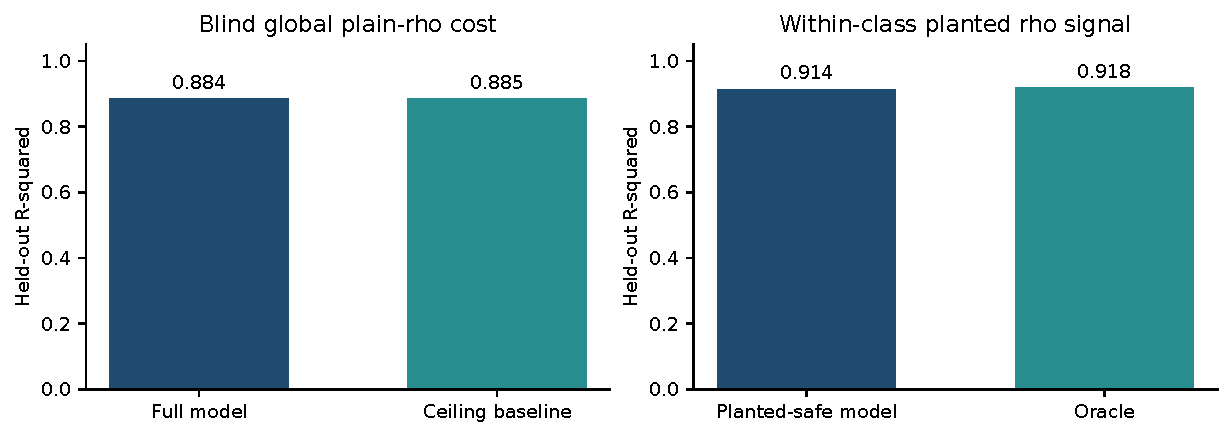
\includegraphics[width=\linewidth]{figures/ml-controls.pdf}
\caption{Why a high prediction score alone is insufficient. Left:
global plain-rho cost is already predicted by the simple ceiling
baseline. Right: a within-class planted structural control is recovered
near its oracle. These are different labels and are not a comparison of
two attack speeds. Recorded M9 values on the isogeny-class split;
source: \src{ML-HARD}.}
\end{figure}

The report also exposes power, split design and feature leakage. A model
using walk-sampling features can learn which node was planted as a root
rather than a transferable mathematical property. A learned policy must
eventually be charged for features, inference, selection and missed
solutions inside a held-out complete pipeline. No such learned component
is shown here to improve the current measured IC frontier.

\subsection{Binary GHS labels vary, but they are formula labels}

The GHS study covers 507 classes and 114,453 nodes over fourteen fields.
It computes exact structural invariants and applies a declared
literature cost formula. The descent label varies within isogeny classes
through the curve coefficient; planted weak nodes and subfield-type
structure are not the same phenomenon.\src{ML-GHS}

On held-out classes, coefficient invariants identify the weak-node label
much better than intrinsic graph features: reported in-class AUCs are
about 0.98 and 0.60. The subfield-degree/endomorphism-level relation has
zero violations on 99,269 checked nodes in the report. These are useful
structural observations and tests of a formula model. They are not
measured complete GHS attack times, and they do not establish a
secret-to-public discovery asymmetry at cryptographic scale.

\subsection{Extension-field degree measurements}

The $\F_{p^n}$ study covers 453 curves over degree-two and degree-three
extensions, with random, subfield, twist, isomorphic and isogenous
families. Its 5,592 target/system rows have Macaulay ranks equal to the
reported regular-sequence values, with the stated solving and
refutation-degree behaviour. It finds target-level degeneracy and
model-over-subfield effects, rather than a general lower degree from
sharing an isogeny class.\src{ML-FPN}

This is evidence about particular formulations over the tested primes.
It should not be pooled with Boolean first-fall experiments as if they
measured the same ideal or the same degree. It also explains why
``isogenous'' and ``same decomposition geometry'' must be distinct
features in a predictive experiment.

\subsection{Symbolic discovery with exact follow-up}

The Smith genus-three programme constructs and studies rational
$(2,2,2)$-isogeny mechanisms on 140,000 random squarefree octics. Its
observed density of curves admitting the declared rational isogeny is
0.1864, with interval [0.1843,0.1884], near the cited prediction 0.1857.
It separately tests trigonal-map rationality, isogeny rationality and
independence across pairings.\src{ML-SMITH}

The rule miner searches products of explicit quadratic-character
features and evaluates candidates on held-out primes and label
permutations. The follow-up twist-bit report has 5,811 certified
nondegenerate cases with no counterexample to the stated character law;
266 trace-zero cases are explicitly not certified by that point-count
criterion. Algebraic identities are checked on additional large-prime
panels. This is much stronger than reporting a classifier score, because
it produces a readable candidate rule and a certificate boundary.
Finite validation remains distinct from a proof for all permitted
curves.\src{ML-TWIST}

The Humbert-surface work recovers equations for $H_4,H_5,H_8,H_{12},H_{13}$
from structured source points, checks them against published equations,
and tests fresh primes. The recorded least weights are 30, 24, 60, 120
and 120 in the chosen invariant presentation. This is a successful
rediscovery and validation workflow, not a priority claim for new
Humbert equations. It also corrects an overgeneralisation: rational real
multiplication in a particular family cannot be inferred for every
point of a Humbert surface from the residue symbol $(D/p)$ alone.
\src{ML-HUMBERT}

\subsection{Assessment of the learning leads}

The most useful learning output so far is an instrument for generating
explicit, falsifiable structural candidates and then removing leakage
and simple explanations. The main hardness-prediction result is
negative beyond the known baselines at the measured scale; the symbolic
and planted-control results are positive within their declared tasks.
Future learning should target a concrete complete-method decision, such
as a base or solver policy whose feature cost is charged, rather than a
large global $R^2$ with no effect on ECDLP work.
